
\chapter{人体姿态估计中的几何约束}

为了实现准确度更高的3D人体姿态估计的目标,引入几何约束可以有效地提升识别准确率,关键在于如何对人体姿态做合理化的定义。因此本章将介绍人体骨骼模型和几种常见的人体参数化表示,结合图像传感器的成像原理,介绍几个成像坐标系的转换原理。

\section{人体姿态表示}
目前在基于深度学习的3D人体姿态估计方法中常见的人体表示法有两种,一种是基于骨骼关节的点线表示法,后一种是基于固定点的姿态表示法。

\subsection{基于骨骼关节的点线表示法}

作为一种常见的人体姿态表示法,就是借助一些传感器,例如Kinect摄像头来捕捉人体三维骨骼关节点的坐标信息。就是将人体所有的关节点看作一个点,而骨骼则就是这些关节点之间的连线。至于两个点之间的角度,自由度之类的,则也可以做部分描述。这样的点线表示法,在本质上而言,就只有两个相邻的关节点才会产生一定的关联。因此在做人体姿态估计的任务时,只能够以平均关节点误差的测量指标作为衡量参数。

\subsection{基于固定点的姿态表示法}

基于固定点的关键在于,如何找到一个合适的关节点,这个关节点需要满足这个条件:其位置变化在人体整体的位置范围中是最小的。目前主要有两种形式,一种是星形结构,目前应用效果不太行,另外一种就是树形结构,能够很好地从选定好的根节点来描述人体姿态,如图~\ref{human_pose_2}所示,\citing{谢子威2019基于深度学习的}图中使用的稳定点为骨盆,对于其他关节点而言,骨盆就是汇聚的终点。

\begin{figure}[h]
	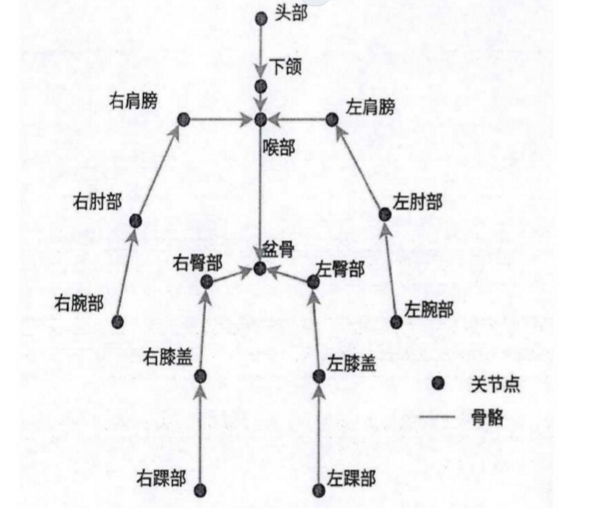
\includegraphics[width=\textwidth]{pic/human_pose_2.jpg}
	\caption{固定点表示示意图}
	\label{human_pose_2}
\end{figure}

\section{人体参数化表示}

人体姿态定义是指人体自身结构呈现的姿态,采用了树形结构\citing{陈明基于混合部件模型的姿态估计方法研究},它规定部件的位置在某个给定的根坐标下是相互独立的。从视觉上来说,用线段表示人体骨架,用点来抽象表示人体主要关节如盆骨,头,胸部,每个关节点都拥有属于各自平移和旋转的自由度,如果需要对各骨骼长度和关节角度的关系进行约束,需要借助人体解刨学的统计数据。这样一来,所有关节点的空间位置可以用以下表示。

\begin{equation}
M = \left[ {\begin{array}{*{20}{c}}
{{x_1}}&{...}&{{x_N}}\\
{{y_1}}&{...}&{{y_N}}\\
{{z_1}}&{...}&{{z_N}}
\end{array}} \right] \in {R^{N \times 3}}
\end{equation}

N为人体关节点数目。由于关键在于对人体自身姿态的分析,所以主要关注人体在三维空间中的相对姿态,在有固定关节点的位置坐标系下,基于与其他关节点之间的位置联系,重建人体三维姿态信息。

\section{误差度量}

对于人体骨骼关键点算法来说,如何有效的衡量一个算法的好坏非常重要,它不像分类问题那样可以很容易采用一些常用指标,例如precise、error、F-score等进行计算。因为在衡量的过程中,我们无法有效的将预测结果与真实值一一对应,无法知道他们之前的对应关系,更加无法知道当前的某个预测结果是否出现了误检或者漏检的情况。因此,构建一个合适的人体关键点的度量指标很重要。

\subsection{OKS}

目前最为常用的就是目标关键点相似性OKS(Object Keypoint Similarity)这个指标,启发于目标检测中的IoU指标,其目的就是为了计算真值和预测人体关键点的相似度。

\begin{equation}
OK{S_p} = \frac{{\sum {_i{e^{ - \frac{{d_{pi}^2}}{{2S_p^2\sigma _i^2}}}}\delta \left( {{v_{pi}} = 1} \right)} }}{{\sum {_i\delta \left( {{v_{pi}} = 1} \right)} }}
\end{equation}

其中:p表示真实值中人的id,I 表示关键点的id,$d_{pi}$表示真实值中每个人和预测的每个人的关键点的欧氏距离,$S_p$表示当前人的尺度因子,这个值等于此人在真实值中所占面积的平方根,即$\sqrt {\left( {{x_2} - {x_1}} \right)\left( {{y_2} - {y_1}} \right)}$,${\sigma _i}$表示第i个骨骼点的归一化因子,因此这个是通过对数据集中所有真实值计算的标准差而得到的,反映出当前骨骼点标注时候的标准差,${\sigma _i}$越大表示这个点越难标注。$v_pi$代表第p个人的第i个关键点是否可见。

\subsection{OKS矩阵}

上面介绍的OKS是计算两个人之间的骨骼点相似度的,那一张图片中有很多的人时,该怎么计算呢?这时候就是构造一个OKS矩阵了。假设一张图中,一共有M个人(groudtruth中),现在算法预测出了N个人,那么我们就构造一个M×N的矩阵,矩阵中的位置(i,j)代表groudtruth中的第i个人和算法预测出的第j个人的OKS相似度,找到矩阵中每一行的最大值,作为对应于第i个人的OKS相似度值。

\subsection{AP(平均准确率)}
此指标用于计算测试集的精度百分比,单人姿态估计和多人姿态估计的计算方式不同。

单人姿态估计,一次仅对一个行人进行估计,即在OKS指标中M=1,因此一张图片中groundtruth为一个行人(GT),对此行人进行关键点检测后会获得一组关键点(DT),最后会计算出GT与DT的相似度OKS为一个标量,然后人为的给定一个阈值T,然后可以通过所有图片的oks计算AP。即假设OKS一共有100个,其中大于阈值T的共有30个,那么AP值就是30/100=0.3.

\begin{equation}
AP = \frac{{\sum\limits_p {\delta \left( {OK{S_p} > T} \right)} }}{{\sum\limits_p 1 }}
\end{equation}

对于多人姿态估计,如果采用的检测方法是自顶向下,先把所有的人找出来再检测关键点,那么其AP计算方法如同单人姿态估计AP。如果采用的检测方法是自底向上,先把所有的关键点找出来然后再组成人,那么假设一张图片中共有M个人,预测出N个人,由于不知道预测出的N个人与groundtruth中的M个人的一一对应关系,因此需要计算groundtruth中每一个人与预测的N个人的OKS,那么可以获得一个大小为M*N的矩阵,矩阵的每一行为groundtruth中的一个人与预测结果的N个人的OKS,然后找出每一行中OKS最大的值作为当前GT的OKS。最后每一个GT行人都有一个标量OKS,然后人为的给定一个阈值T,然后可以通过所有图片中的所有行人计算AP:

\begin{equation}
AP = \frac{{\sum\limits_m {\sum\limits_p {\delta \left( {OK{S_p} > T} \right)} } }}{{\sum\limits_m {\sum\limits_p 1 } }}
\end{equation}

\subsection{PCK}

PCK(Percentage of Correct Keypoints)正确估计出的关键点比例。这是比较老的人体姿态估计指标,在2017年比较广泛使用,作为工程项目使用来评价训练的模型好坏还是蛮方便的。

\begin{equation}
PCK_i^k = \frac{{\sum\limits_p {\delta \left( {\frac{{{d_{pi}}}}{{d_p^{def}}} \le {T_k}} \right)} }}{{\sum\limits_p 1 }}
\end{equation}

其中:I表示id为i的关键点,k表示第k个阈值,p表示第p个行人,$d_pi$表示第p个人中id为i的关键点预测值与人工标注值的欧式距离。$d_p^{def}$表示第p个人的尺度因子,此因子不同公开数据集使用的计算方法不一样,FLIC数据集是以当前人的躯干直径作为尺度因子,即左肩到右臀的欧式距离或者右键到左臀的欧式距离;MPII数据集是以当前人的头部直径作为尺度因子,即头部的左上点与右下点的欧式距离,使用此尺度因子的姿态估计指标也称PCKh。$T_k$是人工设定的阈值。

\subsection{MPJPE}

MPJPE(Mean Per Joint Position Error)平均每关节位置误差,是3D人体姿态估计中最常用的评价指标,每关节的位置误差是一个关节的Groundtruth和预测值之间的欧几里德距离,该种度量方法能够在空间上直观的表现出预测值与真值之间的误差。

\begin{equation}
MPJPE = \frac{1}{T}\frac{1}{N}{\sum\limits_{t = 1}^T {\sum\limits_{i = 1}^N {\left\| {\left( {J_i^{\left( t \right)} - J_{root}^{\left( t \right)}} \right) - \left( {\widehat J_i^{\left( t \right)} - \widehat J_{root}^{\left( t \right)}} \right)} \right\|} } _2}
\end{equation}

其中T为样本数量,N为关节点的数量。计算单位为mm。

\section{人体姿态估计数据集}

对于人体姿态估计而言,目前采用的照片数据集主要分为两类:2D数据集,3D数据集

\subsection{2D数据集}

2D人体姿态识别在dataset和model方面都比3D成熟,2Dmodel也有很多户外,自然界的dataset,但是3D的dataset几乎都是室内的的。常见的数据集,如COCO,MPII。

微软团队开发了一个可以用于计算机视觉很多领域地图像数据集COCO,其全名叫做Common Objects in Context。为了满足训练,验证,测试这三流程的需要,COCO数据集中的图像也可以分为训练、验证和测试这三大类。

\begin{table}[h]
    \centering
    \begin{tabular}{c|c|c|c|c|c}
        \hline
         0-鼻子 &  1-脖子 & 2-右肩 & 3-右肘 & 4-右手腕 & 5-左肩\\
        \hline
         6-左肘 &  7-左手腕 & 8-右臀 & 9-右膝盖 & 10-右脚踝 & 11-左臀\\
        \hline
         12-左膝盖 &  13-左脚踝 & 14-右眼 & 15-左眼 & 16-右耳朵 & 17-左耳朵\\
        \hline
    \end{tabular}
    \caption{COCO标注}
    \label{COCO}
\end{table}

MPII人体姿势数据集是关节式人体姿势估计评估的最新基准。该数据集包括大约25K张图片,其中有超过40K人的身体关节有注释。这些图像是分类收集人类日常活动的。总体而言,训练集带有前后不带注释的帧。此外,对于测试集,我在研究过程中获得了更丰富的注释,包括身体部位遮挡和三维躯干和头部方向。

\begin{table}[h]
    \centering
    \begin{tabular}{c|c|c|c|c|c}
        \hline
         0-右脚踝 &  1-右膝盖 & 2-右臀 & 3-左臀 & 4-左膝盖 & 5-左脚踝\\
        \hline
         6-盆骨 &  7-胸部 & 8-上颈 & 9-头顶 & 10-右手腕 & 11-右肘\\
        \hline
         12-右肩 &  13-左肩 & 14-左肘 & 15-左手腕 \\
        \hline
    \end{tabular}
    \caption{MPII标注}
    \label{MPII}
\end{table}

\subsection{3D数据集}

在数据处理阶段,3D比2D复杂很多。2D人体姿态识别在数据集和模型方面都比3D成熟,2D模型也有很多户外,自然界的数据集,但是3D的数据集几乎都是室内的的。因为3D标注、识别的复杂,所以需要大量的传感器,摄像头去采集数据。

目前主流的3D数据集是Human3.6M,其图像是由四个摄像头捕捉完成的,分别对11个实验测试对象进行捕捉,动作类别也有60种,如\ref{human_dataset}下图所示:

\begin{figure}[h]
	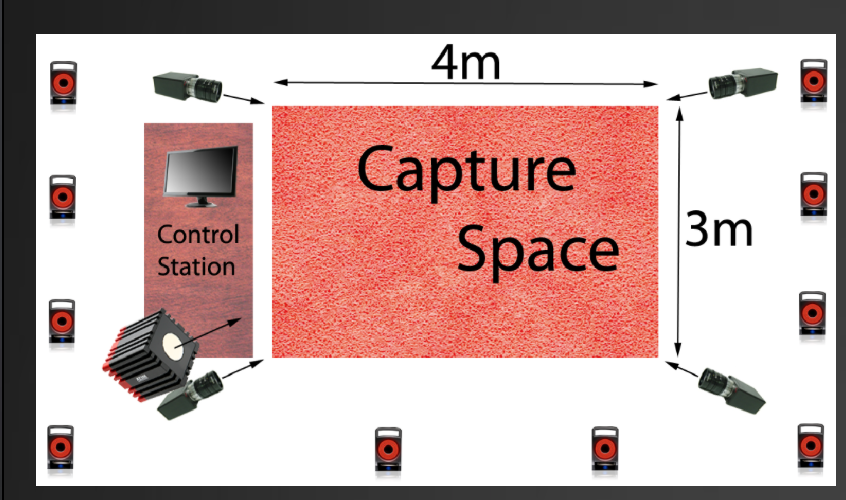
\includegraphics[width=\textwidth]{pic/human_dataset.png}
	\caption{HUMAN3.6M示意图}
	\label{human_dataset}
\end{figure}

由于需要使用该数据集,需要以一个研究机构的名义来申请,且流程极其复杂,所以在本文的研究过程中,只好采用2D数据集,来挖掘其深度信息,最终满足三维人体姿态估计的任务。

\section{成像原理}

图像成像单元在成像过程中扮演着非常重要的作用,因为需要将三维的空间信息映射到二维平面上。因此本节将会介绍,如何提取分析这一个流程的特征信息,以及如何应用于三维人体姿态估计。

\subsection{摄像机模型及其坐标系介绍}

对于一张图片而言,如何从一个三维的立体空间,经过准确的转换,可以以一个较小的信息损失来完成成像任务,这是一个研究内容。将成像流程简略表述如下,即真实物体的空间位置转换到照片成像的几何变化关系。转换过程如\ref{4_para_trans}图所示。

\begin{figure}[h]
	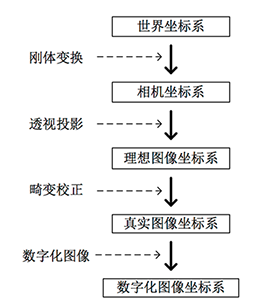
\includegraphics[height=\textwidth]{pic/4_para_trans.png}
	\caption{坐标系转换流程}
	\label{4_para_trans}
\end{figure}

摄像机成像的本质就是将三维空间信息映射到二维平面上的像素信息,而在实际情况下,世界坐标系,摄像机坐标系,成像坐标系以及图像坐标系的相关转换,需要考虑很多因素,比如摄像机的内参以及角度。世界坐标系就是标定点的位置,用毫米(mm)衡量。摄像机坐标系则以相机的光心为原点给出摄像角度的坐标位置,用毫米(mm)衡量。成像坐标系则以摄像机成像平面的坐标位置,用毫米(mm)衡量。图像坐标系则以相机拍摄图片为基准的坐标位置,用像素(mm)来衡量。

\subsubsection{刚体变换(世界坐标系与摄像机坐标系的转换)}

\citing{陈学梅2018基于人体三维姿态的动作评价系统}世界坐标系($X_w,Y_w,Z_w$),是一个三维直角坐标系,可以准确描述相机和待测物体的真实位置。

摄像机坐标系($X_c,Y_c,Z_c$),也是一个三维直角坐标系,镜头光心就是原点,x、y轴分别与相面的两边平行,z轴为镜头光轴,与像平面垂直。

世界坐标系通过旋转矩阵R和平移矩阵T转换得到摄像机坐标系,如图所示,P为空间中的点,其在世界坐标系中表示为$
P\left( {{X_w},{Y_w},{Z_w}} \right)$,在摄像机坐标系中表示$
P\left( {{X_c},{Y_c},{Z_c}} \right)$,三者的坐标系转换关系可用公式表达。

\begin{equation}
\left[ {\begin{array}{*{20}{c}}
{{X_c}}\\
{{Y_c}}\\
{{Z_c}}\\
1
\end{array}} \right] = \left[ {\begin{array}{*{20}{c}}
R&T\\
0&1
\end{array}} \right]\left[ {\begin{array}{*{20}{c}}
{{X_w}}\\
{{Y_w}}\\
{{Z_w}}\\
1
\end{array}} \right]
\end{equation}

\begin{figure}[h]
	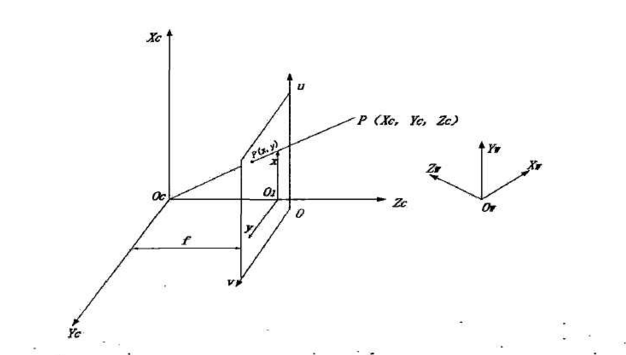
\includegraphics{pic/para_1.png}
	\caption{世界坐标系和摄像机坐标系的转换}
	\label{para_1}
\end{figure}

\subsubsection{透视投影(摄像机坐标系和成像坐标系的转换)}

其实质上就是将三维空同中的点映射成二维平面上的点,将成像平面移到相机光心与物体之间。如图\ref{para_2}所示,$O_c$为摄像机光心点,$O_1$为成像坐标系原点。由空间投影关系可得到公式:

\begin{figure}[h]
	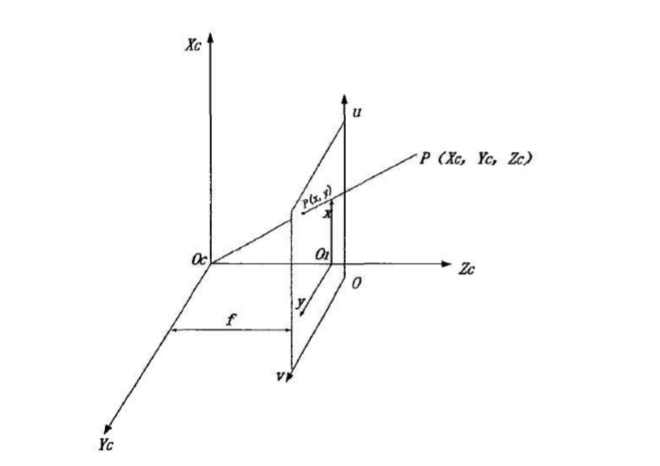
\includegraphics{pic/para_2.png}
	\caption{摄像机坐标系与成像坐标系的转换}
	\label{para_2}
\end{figure}

\begin{equation}
\left\{ {\begin{array}{*{20}{c}}
{x = f\frac{{{X_c}}}{{{Z_c}}}}\\
{y = f\frac{{{Y_c}}}{{{Z_c}}}}\\
{z = f\frac{{{X_c}}}{{{Z_c}}}}
\end{array}} \right.
\end{equation}

将上式转换为齐次坐标系表示如下:

\begin{equation}
\left[ {\begin{array}{*{20}{c}}
x\\
y\\
1
\end{array}} \right] = \left[ {\begin{array}{*{20}{c}}
f&0&0&0\\
0&f&0&0\\
0&0&1&0
\end{array}} \right]\left[ {\begin{array}{*{20}{c}}
{{X_c}}\\
{{Y_c}}\\
{{Z_c}}\\
1
\end{array}} \right]
\end{equation}

\subsubsection{二次转换(成像坐标系与图像坐标系的转换)}

成像坐标系和图像坐标系都在成像平面上,只是各自的原点和度量单位不一样。图像坐标系的原点为相机光轴与成像平面的交点,通常情况下是成像平面的中点。通过离散和平移等操作完成转换,离散化得到相应的像素位置,并且将感应到的色彩调整为用数值存储的像素信息。

\begin{figure}[h]
	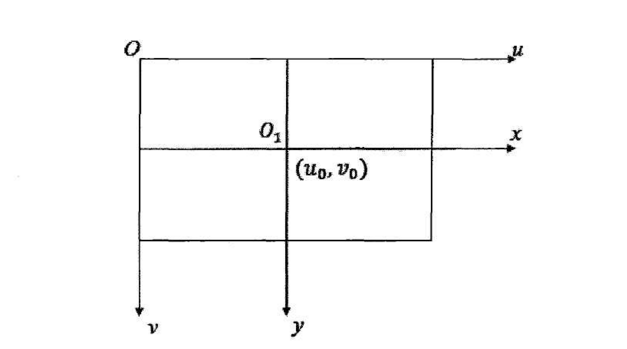
\includegraphics{pic/para_3.png}
	\caption{成像坐标系与图像坐标系的转换}
	\label{para_3}
\end{figure}

如图\ref{para_3}所示,成像坐标系的x,y轴与图像坐标系的u,v轴平行,成像坐标系的原点位于图像坐标系的(${u_0}$,${v_0}$),理想情况下该点位于图像的中心点。二者的关系可用表示:

\begin{equation}
u = \frac{x}{{dx}} + {u_0},v = \frac{y}{{dy}} + {v_0}
\end{equation}

其中dx,dy表示图像中像素间的物理尺寸,转换成齐次坐标系表示为:

\begin{equation}
{Z_c}
\left[          
  \begin{array}{c}   
    u \\
    v \\
    1
  \end{array}
\right]
=
\left[          
  \begin{array}{ccc}   
    1/dx & 0 & {u_0} \\
    0 & 1/dy & {v_0} \\
    0 & 0 & 1
  \end{array}
\right]
\left[          
  \begin{array}{cccc}   
    f & 0 & 0 & 0 \\
    0 & f & 0 & 0 \\
    0 & 0 & f & 0
  \end{array}
\right]
\left[          
  \begin{array}{cc}   
    R & T \\
    0 & 0 
  \end{array}
\right]
\left[          
  \begin{array}{c}   
    {X_w} \\
    {Y_w} \\
    {Z_w} \\
    1 
  \end{array}
\right]
\end{equation}

\begin{equation}
=
\left[          
  \begin{array}{cccc}   
    {f_x} & 0 & {u_0} & 0 \\
    0 & {f_y} & {v_0} & 0 \\
    0 & 0 & 1 & 0
  \end{array}
\right]
\left[          
  \begin{array}{cc}   
    R & T \\
    0 & 0 
  \end{array}
\right]
\left[          
  \begin{array}{c}   
    {X_w} \\
    {Y_w} \\
    {Z_w} \\
    1 
  \end{array}
\right]
\end{equation}

\begin{equation}
=
\left[          
  \begin{array}{cc}   
    M & 0
  \end{array}
\right]
\left[          
  \begin{array}{cc}   
    R & T \\
    0 & 0 
  \end{array}
\right]
\left[          
  \begin{array}{c}   
    {X_w} \\
    {Y_w} \\
    {Z_w} \\
    1 
  \end{array}
\right]
\end{equation}

其中,M为相机内参矩阵,只与相机本身结构有关,记为:

\begin{equation}
M = \left[ {\begin{array}{*{20}{c}}
{{f_x}}&0&{{u_0}}\\
0&{{f_y}}&{{v_0}}\\
0&0&1
\end{array}} \right]
\end{equation}

其中,${f_x} = \frac{f}{{dx}},{f_y} = \frac{f}{{dy}}$表示$u,v$轴的尺度因子。$
\left[ {\begin{array}{*{20}{c}}
R&T\\
0&1
\end{array}} \right]$是相机的外参矩阵,是相机在世界坐标系的位置,M的值与相机的位置摆放有关。

\section{2D热图}

传统的卷积神经网络来回归人体关键节点坐标的方法,其实并不能实现精准定位,目前的研究\cite{zhang2019distributionaware}中,采用回归热力图才能得到较高水平,这是因为热力图的本质就是概率图,图中的高斯峰值处,就是预测到的关节位置出现概率最大的位置坐标。为了使得热力图标签能和对应的目标对象不发生错乱,所以必须要分配好不同的热力图标签。

其生成公式如下:

\begin{equation}
G\left( {i,j} \right) = \frac{1}{{\sqrt {2\pi {\delta ^2}} }}{e^{\frac{{{{\left( {i - \widetilde x} \right)}^2} + {{\left( {j - \widetilde y} \right)}^2}}}{{2{\delta ^2}}}}}
\end{equation}

在这里我们假设,$i = 1,2,...,\widetilde w$,$j = 1,2,...,\widetilde h$可以表示热力图的空间位置变化,(i,j)是人体关节点的位置坐标,$ \left( {\widetilde x,\widetilde y} \right) $对应(x,y)在热力图中的位置, $ \delta $是控制高斯分布函数的参数(上图中亮斑的半径)。热力图尺寸一般小于原图尺寸,假设热力图的尺寸是原图像尺寸的1/p倍,则 $ \left( {\widetilde x,\widetilde y} \right) $人体关键点坐标也将会对应地缩小1/p倍,$ 
\left( {\widetilde w,\widetilde h} \right)$是原图尺寸(w,h)也将会缩小1/p倍。
关于人体姿态的十六个关节点的识别则根据热力图进行判断,如图\ref{heatmap}所示,显示出来亮斑的地方就是关节点概率最大的位置。

因此热力图的目标就是预测给定输入图像中的关节坐标。为此,我们需要借助之前第二章所提到的沙漏模型,在模型训练和测试期间,热力图经常被用作坐标表示。\cite{zhang2019distributionaware}具体来说,我们假设可以访问一组训练图像。为了便于模型学习,我们将标注的关节地真坐标编码成热图作为有监督的学习目标。在测试过程中,我们需要将预测的热图解码成原始图像坐标空间中的坐标。

\begin{figure}[h]
	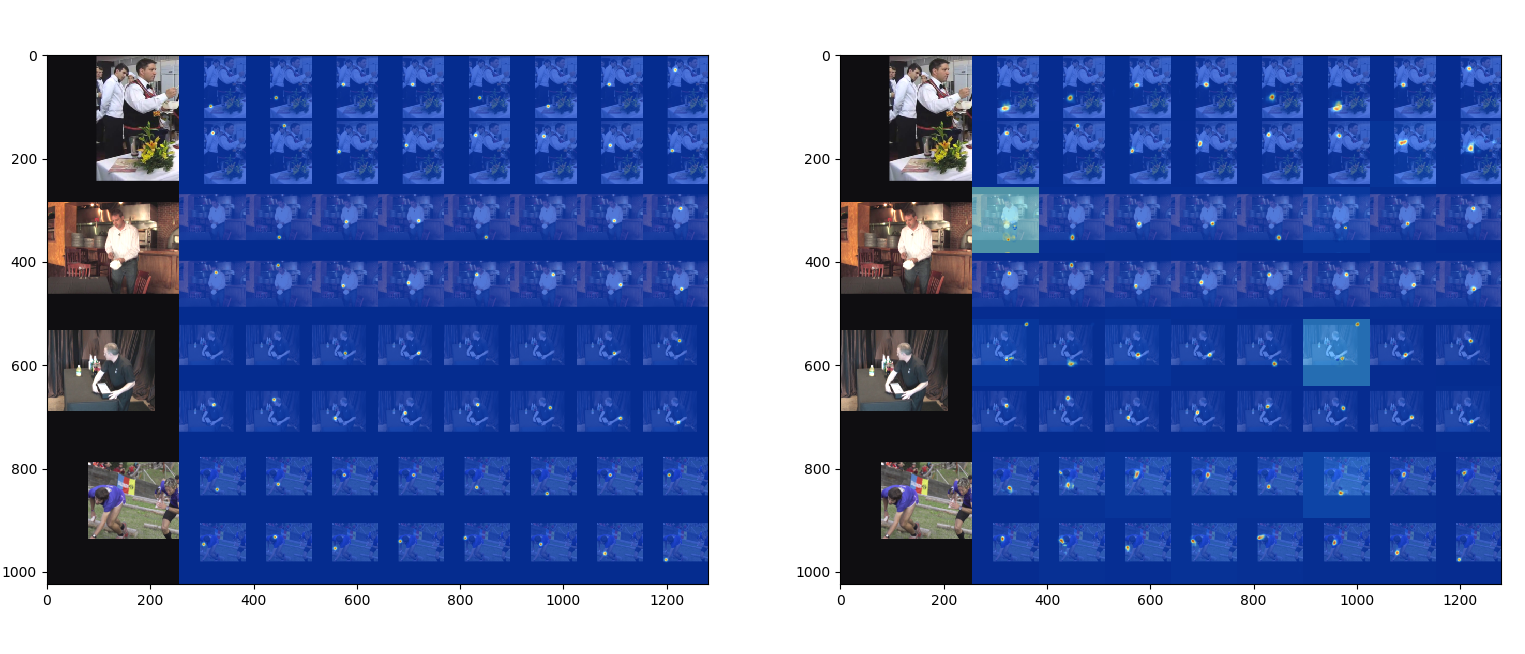
\includegraphics[width=\textwidth]{pic/screenshot.png}
	\caption{2D热力图演示}
	\label{heatmap}
\end{figure}

\section{深度回归模块}

根据一些相关文献,一般而言,2D的前两维坐标相较于而言,识别精度较高,而对于第三维坐标(Z),识别的误差较大,所以设计一款深度回归模块,用于更好地得到第三维坐标,提高3D人体姿态估计的精度。

\subsection{针孔成像原理}

对于针孔成像模型,我们这里做出如下推导。在该图中,绿色箭头和蓝色箭头分别代表以x轴和y轴为中心的关键点的坐标。而黄线代表的是射线,c代表针孔。$d,f,l_{sensor}$代表的是相机与人的关键点之间的距离(mm),焦距(mm),在图像坐标系上的人的长度(mm)。根据tan的定义,我们可以得到如下推导。

\begin{figure}[h]
	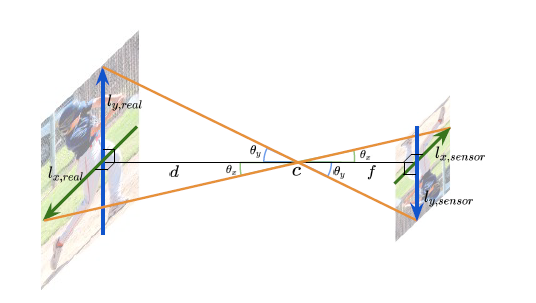
\includegraphics{pic/depth.png}
	\caption{针孔成像原理}
	\label{depth}
\end{figure}

\begin{equation}
\tan {\theta _x} = \frac{{0.5{l_{x,real}}}}{d} = \frac{{0.5{l_{x,sensor}}}}{f}
\end{equation}

其中,我们做出假设$p_x,p_y$成为指定坐标系的像素距离参数因子,然后可以得到

\begin{equation}
d = f\frac{{{l_{x,real}}}}{{{l_{x,sensor}}}} = f{p_x}\frac{{{l_{x,real}}}}{{{l_{x,sensor}}{p_x}}} = {\alpha _x}\frac{{{l_{x,real}}}}{{{l_{x,img}}}}
\end{equation}

同理可得,在y轴上也适用

\begin{equation}
d = f\frac{{{l_{y,real}}}}{{{l_{y,sensor}}}} = f{p_y}\frac{{{l_{y,real}}}}{{{l_{y,sensor}}{p_y}}} = {\alpha _y}\frac{{{l_{y,real}}}}{{{l_{y,img}}}}
\end{equation}

所以这里我们做一个假设,认为d和x,y轴的参数因子都有关系。
结合前面两个式子,可以得到,

\begin{equation}
d = \sqrt {{\alpha _x}{\alpha _y}\frac{{{l_{x,real}}}}{{{l_{x,img}}}}\frac{{{l_{y,real}}}}{{{l_{y,img}}}}}  = \sqrt {{\alpha _x}{\alpha _y}\frac{{{A_{real}}}}{{{A_{img}}}}} 
\end{equation}

其中${\alpha _x}$,${\alpha _y}$分别代表焦距在x,y轴上的像素参数,${A_{img}}$代表图片的像素大小,单位为
$pixe{l^2}$。${A_{real}}$代表真实空间中大小,单位为$mm{l^2}$。

然而,通过针孔成像的模型得到的深度值并一定是实际的深度值,这是因为,由于${A_{img}}$是通过扩展2D边界框而获得的,因此尽管与摄像机的距离相同,但其外观可能会有所不同。例如,如图\ref{depth_ambiguity}的左图所示,尽管两个人到相机的距离相同,但他们的${A_{img}}$不同。 另一方面,在某些情况下,即使距相机的距离不同,${A_{img}}$也可以相同。 例如,在图\ref{depth_ambiguity}的右图中,儿童和成人的${A_{img}}$相似,但是,儿童比成人更靠近相机。

\begin{figure}[h]
	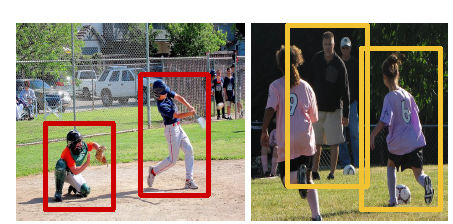
\includegraphics{pic/depth_ambiguity.png}
	\caption{深度表现的歧义性}
	\label{depth_ambiguity}
\end{figure}

根据[1]得到的图\ref{k_depth}关于d和真实的深度值的关系,呈现如下的相关性。

\begin{figure}[h]
	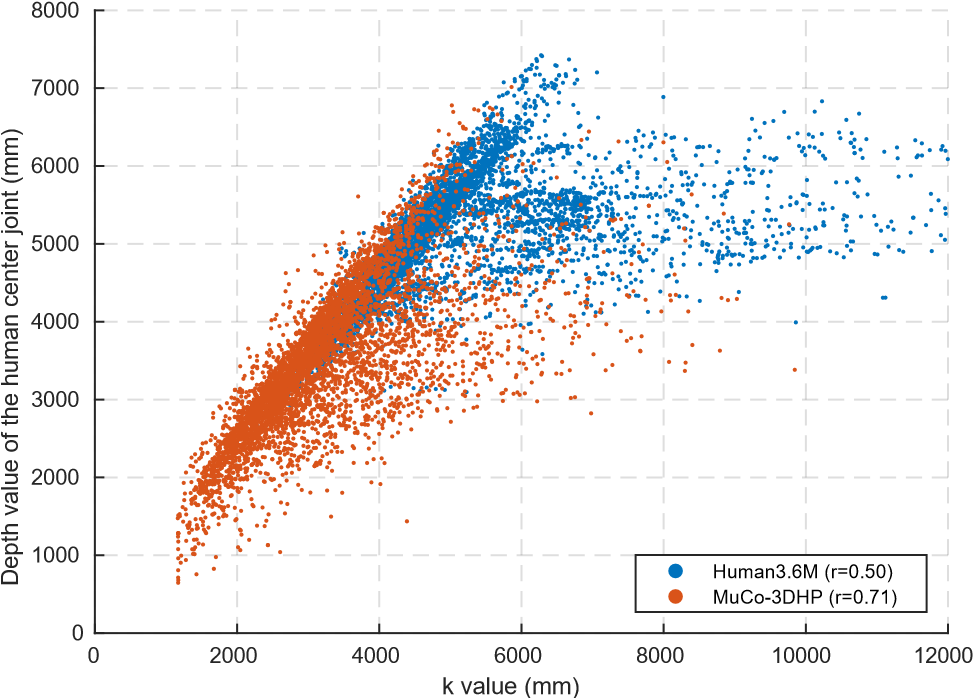
\includegraphics{pic/k_depth.png}
	\caption{k值与实际深度值的相关性。使用了人类3.6M数据集和MuCo-3DHP数据集。r表示皮尔逊相关系数。}
	\label{k_depth}
\end{figure}

为解决此问题,我们设计了矫正因子这么一个概念,以利用图像功能纠正${A_{img}}$,最终纠正d。 图像可以为深度回归提供有关${A_{img}}$必须更改多少的线索。例如,在图中\ref{depth_ambiguity},左图可以告诉深度回归增加面积,因为人类处于蹲伏状态。同样,在图\ref{depth_ambiguity}中,正确的图像可以告诉深度回归模块增加区域,因为输入图像包含一个子对象。 具体而言,深度回归模块从图像特征输出校正因子
$ \gamma$。 估计的
$ \gamma$乘以给定${A_{img}}$,即为
$ \gamma {A_{img}}$。 根据$ \gamma {A_{img}}$,计算出k,它成为最终的深度值。

结合上述的针孔成像原理,我们在这里,为简化讨论,我们设计如下模块

其算法思路如图\ref{k_depth_model}所示:

\begin{figure}[h]
	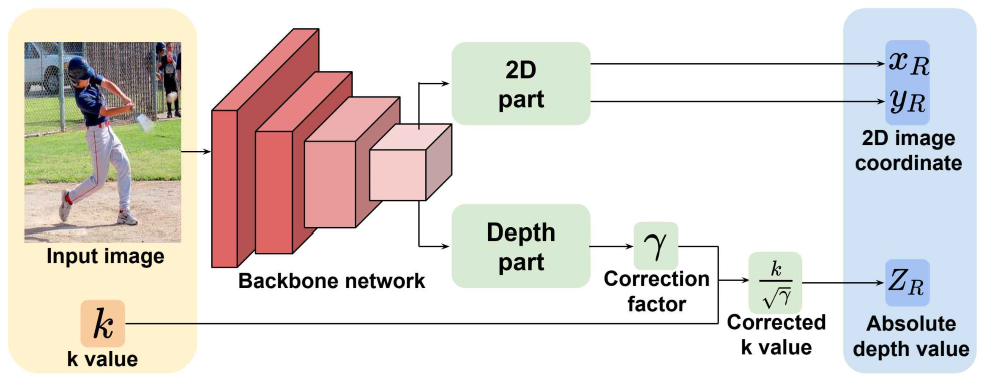
\includegraphics[width=\textwidth]{pic/K_depth_model.png}
	\caption{深度回归模块设计}
	\label{k_depth_model}
\end{figure}

网络架构包括三个组件,如图所示。首先,骨干网提取输入的人类图像的有用的全局特征。其次,二维图像坐标估计部分从骨干部分获取特征图,并使用具有批处理归一化层的三个连续卷积层和ReLU激活函数对其进行上采样。然后,1*1卷积网络被用于产生2D热图,Softargmax从2D热图提取2D图像坐标$x_R,y_R$。第三部分是深度估计部分。它还从主干部分获取特征映射,并应用全局平均池。然后,合并的特征映射经过1乘1卷积,该卷积输出单个标量值γ。最后的绝对深度值$Z_R$是通过乘以k得到的。

\section{人体姿态估计思路}

基于单目图像的三维人体识别算法按照方法可以分为两类:1.基于两阶段的三维人体姿态识别,2.基于端到端的三维人体姿态识别。

\subsection{基于两阶段的三维人体姿态识别}

基于两阶段的三维人体姿态识别,意味着计算机首先从二维RGB图像中提取人体骨架并估计其二维位置,然后根据二维骨架信息预测三维骨架的空间位置。由于二维骨架信息是三维人体姿态识别的重要输入,所以二维人体姿态识别的准确率较大地影响着三维人体识别的误差。Yang和Ramanan\citing{Yang2011}改进该模型,不采用链接式人体躯干部分,而是使用每个身体部位的混合模板来捕获部位之间的上下文共现关系,体现了局部刚性的概念。之前的工作要么使用偏离某个模板的局部可变形模型,要么在人体姿态空间中使用全局混合表示方法。

\subsection{基于端到端的三维人体姿态识别}

基于端到端的三维人体姿态识别表示在给定的图像或者视频下,将其作为输入直接输出人体骨骼关键点在三维空间中的位置。Tekin\citing{DBLP:journals/corr/TekinKSLF16}使用深度学习回归架构,用于单目图像的3D人体姿势结构化预测,该架构通过自动编码器来学习高维潜在姿态表示方法并解释关节依赖性,对人体姿态添加隐式约束。由于\citing{DBLP:journals/corr/TekinKSLF16}只是简单地将每个关节的位置误差最小化,而忽略了姿态的内部结构,Sun\citing{sun2017compositional} 使用骨骼代替关节作为姿势表示方法,并利用关节连接结构对骨骼之间的远程相互作用进行编码。Pavlakos\citing{DBLP:journals/corr/PavlakosZDD16} 为改善关节坐标的直接回归性能,首先需要对人体周围的3D空间进行离散化,
这是为了使得训练的ConvNet,可以很好地预测每个关节位置的可能性。为了自然图像中2D和3D人体姿态联合估计,Rogez\citing{8099617}提出一种用于的网络LCR-Net,不需要对图中进行近似定位,仅需在每个图像生成多个姿态提案和对其计分,最终的姿态估计是通过对相邻姿态假设进行积分而获得的。Tekin\citing{DBLP:journals/corr/TekinMSF16}为结合从图像直接回归到3D关节坐标和从2D关节位置推断3D坐标的优点,引入了判别式融合框架,以同时利用2D关节位置置信度图和3D图像提示进行3D人体姿势估计,并且提供了一种可训练的融合方案,该方案可自动学习在何处以及如何融合这两种信息源。

根据国内外研究现状所知,虽然基于两阶段的三维人体姿态识别方法在一定程度上取决于二维姿态检测器的性能,但是与基于端到端的三维人体姿态识别相比,其可以在不同的无对应关系的数据库分开训练二维、三维姿态检测器,不因只存在2D标注而无对应的3D标注的野外图像数据限制,可训练数据范围更广,训练方式更加多样化。因此,本文采用的是基于两阶段的三维人体姿态识别方法。

\section{整体算法框架设计思路}

本文算法采用两阶段的3D人体姿态估计算法,即第一步,使用骨干网络(堆叠沙漏网络)提取2D热图,根据2D热图的峰值点,即可判定于前两个坐标的最大概率位置。而第三维则采取上一节设计的深度回归模块,用来提取第三维特征,根据不同的校正因子,可以进行不同的校正作用,总之目的就是减少误差。
 
因此,整个网络架构具体设计如图所示\ref{depth_model},包括三个组件。首先,骨干网提取输入的人类图像的有用的全局特征。其次,二维图像坐标估计部分从骨干部分获取特征图,并使用具有批处理归一化层的三个连续卷积层和ReLU激活函数对其进行上采样。然后,1*1卷积网络被用于产生2D热图,Softargmax从2D热图提取2D图像坐标$x_R,y_R$。第三部分是深度估计部分。它还从主干部分获取特征映射,并应用全局平均池。然后,合并的特征映射经过1乘1卷积,该卷积输出单个标量值γ。最后的绝对深度值$Z_R$是通过乘以k得到的。

\begin{figure}[h]
	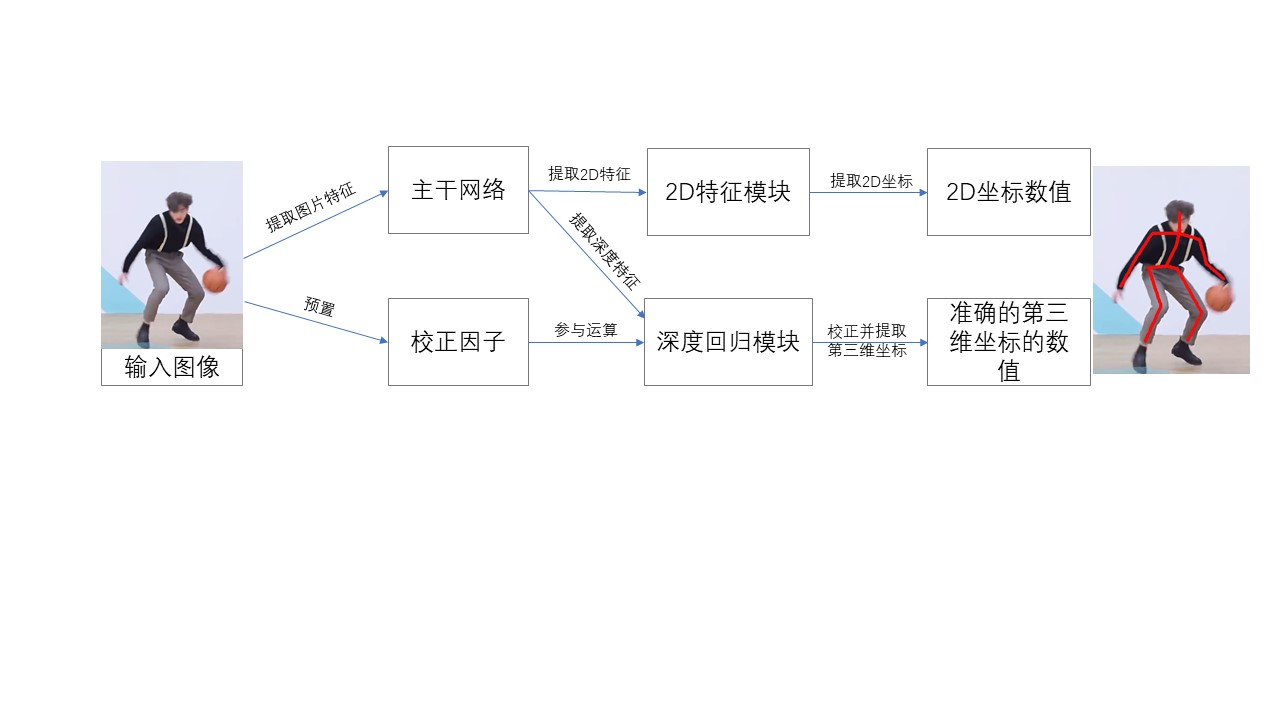
\includegraphics[width=\textwidth]{pic/depth_model.jpg}
	\caption{整体模块设计}
	\label{depth_model}
\end{figure}

\section{本章小结}
本章介绍了人体姿态估计涉及到的基本概念,并简单分析了两种常见人体姿态表示法,还有衡量人体姿态估计算法优劣的误差度量,以及目前学术界主流数据照片集的标注方法。并且介绍了摄像单元的成像原理,并结合单孔成像原理,设计了一个深度回归模块,用于提升整个算法框架。